\documentclass[aoas,preprint, 11pt, dvipsnames, table, x11name]{imsart}

% natbib citation styles, see the natbib documentation, a copy of which
\usepackage{tikz-cd}
\usepackage[toc,page]{appendix}
\usepackage[font={small}, labelfont=bf]{caption}
\usepackage{subcaption}
\usepackage[utf8]{inputenc}
\newcommand{\E}{\mbox{E}}
\newcommand{\N}{\mbox{N}}
\usepackage{amsfonts}
%Font
\usepackage[T1]{fontenc}
\usepackage{comment}
%\usepackage[dvipsnames,table,x11names]{xcolor}
\usepackage{xcolor}
\definecolor{darkgreen}{RGB}{0,69,0} %for rf
\definecolor{navy}{RGB}{0,60,113} %tough choice
\usepackage{booktabs}
\usepackage{bbm}
\usepackage{array}
\newcolumntype{P}[1]{>{\centering\arraybackslash}p{#1}}
\newcolumntype{P}[1]{>{\centering\arraybackslash}p{#1}}

\setlength{\parskip}{\baselineskip}
\usepackage{imakeidx}
\usepackage{tikz}
\usetikzlibrary{arrows.meta, calc, positioning}
%\usetikzlibrary{arrows}
\usetikzlibrary{positioning}
\newdimen\nodeDist{}
\nodeDist=25mm
\usepackage{pgfplots}
\newcommand{\indep}{\rotatebox[origin=c]{90}{$\models$}}
%\usepackage[english]{babel}
\usepackage{graphicx}
\graphicspath{{../figures/}}
\usepackage{amsmath,commath,amssymb,blkarray,bm,bbm}
\usepackage{bbm}
\usepackage{mathtools}
\newcommand{\imp}[1]{\textbf{#1}}
\renewcommand{\bm}[1]{\mathbf{#1}}
\usepackage{mathrsfs}
\usepackage{physics}
\usepackage[pagebackref]{hyperref}  
\usepackage{comment}
\usepackage[authoryear]{natbib}
\bibliographystyle{plainnat}
\newcommand\independent{\protect\mathpalette{\protect\independenT}{\perp}}
\def\independenT#1#2{\mathrel{\rlap{$#1#2$}\mkern2mu{#1#2}}}
\DeclareMathOperator{\NA}{NA}
\newcommand{\ind}[1]{\mathbbm{1}({#1})}%
\hypersetup{
	colorlinks=true,
	linkcolor={blue},
	filecolor=magenta,      
	urlcolor={blue},
	citecolor={blue}
}
\bibliographystyle{imsart-nameyear}
\urlstyle{same}
%% Packages
\RequirePackage{amsthm,amsmath,amsfonts,amssymb}
\RequirePackage[authoryear]{natbib}
%\RequirePackage[colorlinks,citecolor=blue,urlcolor=blue]{hyperref}
%\RequirePackage{graphicx}

\startlocaldefs
%%%%%%%%%%%%%%%%%%%%%%%%%%%%%%%%%%%%%%%%%%%%%%
%%                                          %%
%% Uncomment next line to change            %%
%% the type of equation numbering           %%
%%                                          %%
%%%%%%%%%%%%%%%%%%%%%%%%%%%%%%%%%%%%%%%%%%%%%%
%\numberwithin{equation}{section}
%%%%%%%%%%%%%%%%%%%%%%%%%%%%%%%%%%%%%%%%%%%%%%
%%                                          %%
%% For Axiom, Claim, Corollary, Hypothezis, %%
%% Lemma, Theorem, Proposition              %%
%% use \theoremstyle{plain}                 %%
%%                                          %%
%%%%%%%%%%%%%%%%%%%%%%%%%%%%%%%%%%%%%%%%%%%%%%
%\theoremstyle{plain}
\newtheorem{axiom}{Axiom}
\newtheorem{claim}[axiom]{Claim}
\newtheorem{theorem}{Theorem}[section]
\newtheorem{lemma}[theorem]{Lemma}
%%%%%%%%%%%%%%%%%%%%%%%%%%%%%%%%%%%%%%%%%%%%%%
%%                                          %%
%% For Assumption, Definition, Example,     %%
%% Notation, Property, Remark, Fact         %%
%% use \theoremstyle{remark}                %%
%%                                          %%
%%%%%%%%%%%%%%%%%%%%%%%%%%%%%%%%%%%%%%%%%%%%%%
\theoremstyle{remark}
\newtheorem{definition}[theorem]{Definition}
\newtheorem*{example}{Example}
\newtheorem*{fact}{Fact}
%%%%%%%%%%%%%%%%%%%%%%%%%%%%%%%%%%%%%%%%%%%%%%
%% Please put your definitions here:        %%
%%%%%%%%%%%%%%%%%%%%%%%%%%%%%%%%%%%%%%%%%%%%%%

\endlocaldefs


\begin{document}
\section{Estimating the risk difference as estimand of interest}\label{4.4}
Rather than looking at the ratio of potential outcomes, it is often the case we want to investigate the difference in the expected value of each, i.e. we can look at \emph{risk differences}:
\[\text{Risk Difference}\rightarrow \delta \equiv \E(B^1)-E(B^0)\]
In our framework, following similar reasoning as in section \emph{Modular sensitivity analysis with machine learning}in the main file,  risk differences can be defined as 
\[\Delta(\mathbf{x}_i)=\int_{\mathbb{R}} \Phi\qty(b_1(\mathbf{x})+u)f(u)\dd u - \int_{\mathbb{R}} \Phi\qty(b_0(\mathbf{x})+u) f(u)\dd u\]
The sample average risk difference (ARD) is therefore $\frac{1}{n}\sum_{i=1}^{n}\Delta(\mathbf{x}_i)$. In the case of the audit data, the average risk difference refers to percentage point difference in going bankrupt after receiving a going concern. We esimate the risk difference using our methodology as well as the bivariate probit with endogenous regressor model, (described in equation(4) in the main file), to the audit data.  Specifically, we used the same covariates as we used when fitting monotone bart, used the bankruptcy indicator as the binary outcome, and whether or not a going concern was issued as the ``treatment'' indicator.  Using our methodology, results for estimating risk differences on the audit data are presented in table \ref{resultssummary}.


\begin{table}[ht]
	\centering
	%	\scalebox{.9}{
	\begin{tabular}{lllllP{1.5cm}}
		\toprule
		$\gamma$&$\rho$& ARD true & ARD est&IRD cor&IRD RMSE \\ 
		\midrule
		1.00&0.25& 0.29 & 0.29 & 0.89 & 0.05  \\ 
		1.75&0.25& 0.47 & 0.47 & 0.96&0.04  \\ 
		2.50&0.25& 0.58 & 0.57 &  0.97&0.05  \\ 
		1.00&0.40 &0.29 & 0.29 &  0.90&0.05  \\ 
		1.75&0.40& 0.47 & 0.46 &  0.94&0.06  \\ 
		2.50&0.40& 0.58 & 0.55 &  0.96&0.09  \\ 
		1.00&0.60&  0.29 & 0.29 &  0.90&0.05  \\ 
		1.75&0.60& 0.47 & 0.46 &  0.95 &0.05 \\ 
		2.50&0.60& 0.58 & 0.57 & 0.98&0.04  \\ 
		1.00&0.80& 0.29 & 0.27 &  0.91&0.05  \\ 
		1.75&0.80& 0.47 & 0.44 &  0.95 &0.05 \\ 
		2.50&0.80 &0.58 & 0.55 &  0.98&0.05 \\
		\bottomrule
	\end{tabular}
	%}
	
	\caption{We simulate from the bivariate probit with 25,000 observations and deploy our methodology.  cor refers to the correlation between predicted and true for the average risk difference (ARD), and the rmse is the root mean square error. }
	\label{bivartable_treat}
\end{table}

When fitting the bivariate probit regression, parameters are estimated using maximum likelihood. Our ARD from this regression was 2.90 percentage points and a mean risk ratio of 2.82 with 95\% CI (1.33, 6.04).  Note, we used a regression spline approach to smooth our numeric covariates, where the smooth term for each covariate is made of basis functions, see \cite{marra} for details.  This gives us additional flexibility in fitting the model.

\begin{table}[h]
	\centering
	%	\begin{bclogo}[couleur=newblue!74!white, arrondi=0.16, logo=\bcplume ,, ombre=true, barre=none ]{}
	%\begin{tabular}{lllll}%{P{1.6cm}P{1.5cm}P{1.5cm}P{1.5cm}P{1.5cm}P{2cm}}
	\begin{tabular}{lP{1.1cm}P{1.1cm}P{1.1cm}P{2.3cm}}
		%	\toprule
		%	&\color{BrickRed}\textbf{XGBoost}&\color{darkgreen}\textbf{Random Forest}&\color{navy}\textbf{BART}\\ \midrule
		%\multicolumn{2}{c}Method&\multicolumn{2}{c}{\color{BrickRed}{XGBoost}} &\multicolumn{2}{c}{\color{darkgreen}{Random %Forest}}&\multicolumn{2}{c}{\color{navy}{BART}}\\
		%	\midrule
		\toprule
		Distribution of $f(u)$  & ARD (\%)&ARD post (\%)& mean $B_1$ (\%) &95\% Credible interval for ARD (\%)  \\ \midrule
		$\N(0,\sigma=0.1)$ &8.89&8.91&10.3&$\qty(6.95, 11.2)$\\ %\hline
		$\N(0,\sigma=0.5)$ &3.62&3.76 &5.29 &$\qty(2.78, 4.97)$\\%\hline      
		$\N(0,\sigma=1)$&0.41&0.63&2.57&$\qty(0.37, 0.97)$\\
		Shark $q=0.25$, $s=0.5$; $\sigma=1.05$&0.11&0.24&2.44&$\qty(0.13, 0.40)$\\
		Shark $q=0.75$, $s=1.25$; $\sigma=0.88$&2.39&2.57&4.30&$\qty(1.82, 3.52)$\\
		
		``Right Bump'' $\sigma=0.48$&1.98&2.17&4.10&$\qty(1.78, 2.69)$\\
		98\% peak $\sigma=0.29$&6.85&7.08&8.62&$\qty(5.41, 9.06)$\\
		90\% peak $\sigma=0.64$&1.85&2.03&4.02&$\qty(1.68, 2.51)$\\
		%	80\% peak&1.66&4.30&100\\
		
		\bottomrule%\\\midrule %\hline       
		%total&333&435&66&47&& \\ \bottomrule        
	\end{tabular}
	%\captionsetup{labelformat=empty}
	\caption{The reduced form probabilities (equation (15) in the main file) were estimated using BART with a monotonicity constraint on the going concern variable.  We further require $b_1(\bm{x})>b_0(\bm{x})$ in the projection step.  Posterior summaries based on 500 Monte Carlo samples.  $\sigma$ refers to the implied standard deviations of the different distributions.}
	%\caption{LHS of system of equations \ref{long} estimated using BART with monotonicity constraint.  Additional constraint in optimization/integration step requires $b_1(\bm{x})>b_0(\bm{x})$.  Credible interval based on quantiles of random sample of 500 posterior draws.  Interpret the inducement as percentage point increase in probability of bankruptcy.  $\sigma$ in the shark fin refers to implied standard deviation given $q$ and $s$ parameters. The mean $\tau$ column refers to the mean inducement effect calculated by solving the integral formulation of \ref{maineq} once with LHS probabilities given by the mean of the BART posterior estimate. mean $\tau$ post refers to the mean of the inducement effect after solving the system of equations for each 500 posterior draws of the estimates of the LHS probabilities of \ref{maineq}, and mean $B_1$ refers to the mean bankruptcy probability (including the treatment effect).}
	\label{resultssummary}
	%\end{bclogo}
\end{table}


It was stressed in the main document how using  BART with a monotonicity constraint improves our estimation of the ICRR, but the improvement is even more pronounced when studying risk differences.  
In figure \ref{monovsnorm_ITE}, we look at the comparison of IRD (individual risk difference) estimates from data generated by the bivariate probit, with the left hand side of our system of equation probabilites estimated with BART and monotone BART.  This is a similar plot to figure 14 in the main file, but with a different estimand of interest.
\begin{figure}[h]
	\centering
	\begin{subfigure}{.5\textwidth}
		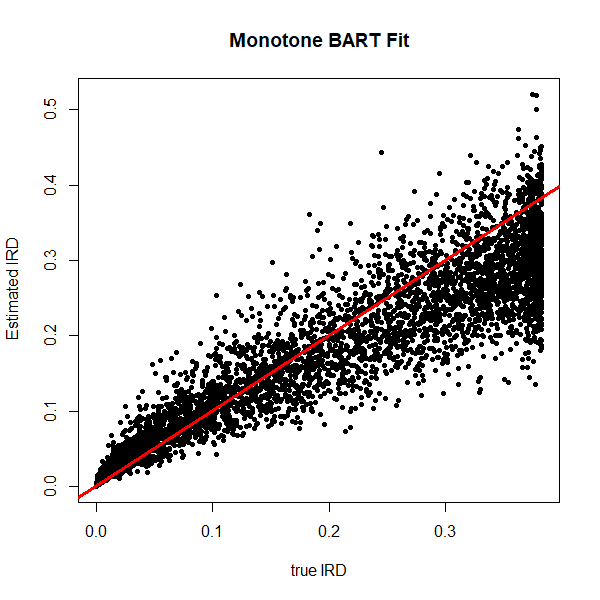
\includegraphics[width=6.cm]{monobartITE_png.png}
	\end{subfigure}%
	\begin{subfigure}{.5\textwidth}
		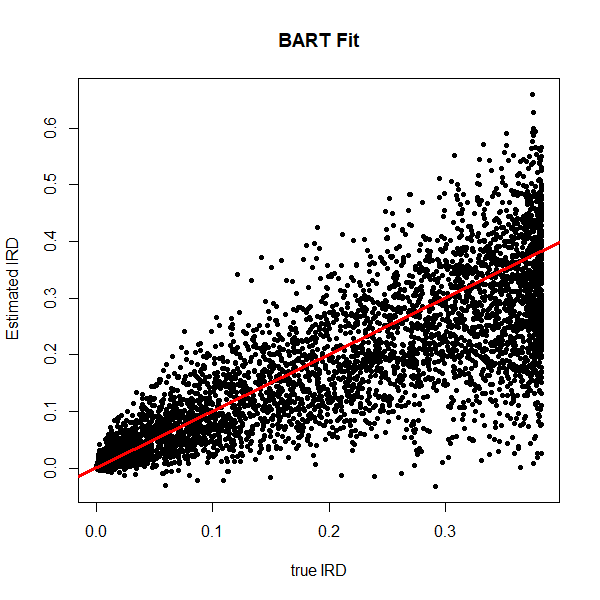
\includegraphics[width=6.cm]{BartITE_png.png}
	\end{subfigure}
	\caption{Plots of expected individual risk differences (IRD) vs our estimates, i.e. a plot comparing the difference in potential outcomes from the bivariate probit model ($\Phi(\alpha_0+\alpha_1\bm{x}_i+\gamma)-\Phi(\alpha_0+\alpha_1\bm{x}_i)$) versus our estimate.  In the DGP, $\rho=0.25,\gamma=1$.  The monotone BART correlation between $\tau$ and $\hat{\tau}$ is 0.928 and for BART is 0.826}
	\label{monovsnorm_ITE}
\end{figure}

\section{Bivariate probit simulation study}\label{bivar_append}
Table \ref{bivarvalidate} shows the results when fitting the bivariate probit regression with a maximum likelihood estimate to the simulated bivariate probit data.  Unsurprisingly, this performs well, with the caveat that we require large $\N$ ($\N=100,000$) to get these impressive results.  We simulated the samples from the bivariate probit model of the main document, where we sum 5 uniform(-1,1) $\bm{x}_i$ covariates each with the same $\beta_1$ and $\alpha_1$ coefficients respectively.  We set $\beta_0=0, \beta_1=-0.2, \alpha_0=-0.5, \alpha_1=0.7$ to generate reasonable number of going concerns and bankruptcies.

Table \ref{bivartable_treat} shows the results when we simulate from the bivariate probit and fit with our methodology, with $f(u)$ assigned appropriately, only this time we are interested in the treatment effect.  Our method does well here, with only $\N=25,000$ and $p=5$.  

\begin{table}[h]
	\centering
	\scalebox{.9}{
		\begin{tabular}{lllP{1.3cm}P{1.3cm}P{1.3cm}P{1.3cm}P{1.3cm}llll}
			\toprule
			ARD true & ARD est&IRD cor&IRD RMSE&ACRR true&ACRR est& ICRR cor&ICRR rmse&  $\gamma$ true&$\gamma$ est.& $\rho$& $\rho$ est. \\ 
			\midrule
			0.23 & 0.24 & 0.97 & 0.02 & 2.24 & 2.07 & 1.00 & 0.24 & 1.00 & 0.77 & 0.25 & 0.37 \\ 
			0.46 & 0.46 & 0.99 & 0.02 & 4.32 & 3.89 & 1.00 & 0.87 & 1.75 & 1.62 & 0.25 & 0.31 \\ 
			0.58 & 0.57 & 1.00 & 0.02 & 6.24 & 5.40 & 0.99 & 2.34 & 2.50 & 2.38 & 0.25 & 0.30 \\ 
			0.26 & 0.26 & 0.99 & 0.01 & 2.42 & 2.27 & 1.00 & 0.22 & 1.00 & 0.85 & 0.40 & 0.47 \\ 
			0.46 & 0.46 & 0.99 & 0.02 & 4.33 & 3.89 & 1.00 & 0.90 & 1.75 & 1.63 & 0.40 & 0.45 \\ 
			0.57 & 0.56 & 0.99 & 0.02 & 6.14 & 5.13 & 1.00 & 2.83 & 2.50 & 2.34 & 0.40 & 0.46 \\ 
			0.28 & 0.28 & 0.99 & 0.01 & 2.57 & 2.46 & 1.00 & 0.17 & 1.00 & 0.92 & 0.60 & 0.63 \\ 
			0.47 & 0.47 & 1.00 & 0.01 & 4.51 & 4.24 & 1.00 & 0.63 & 1.75 & 1.70 & 0.60 & 0.61 \\ 
			0.59 & 0.58 & 1.00 & 0.01 & 6.41 & 5.89 & 0.99 & 1.67 & 2.50 & 2.45 & 0.60 & 0.61 \\ 
			0.31 & 0.31 & 1.00 & 0.00 & 2.79 & 2.80 & 1.00 & 0.02 & 1.00 & 1.02 & 0.80 & 0.80 \\ 
			0.47 & 0.47 & 1.00 & 0.01 & 4.51 & 4.26 & 1.00 & 0.56 & 1.75 & 1.70 & 0.80 & 0.81 \\ 
			0.58 & 0.58 & 1.00 & 0.01 & 6.31 & 5.56 & 0.99 & 2.25 & 2.50 & 2.41 & 0.80 & 0.82 \\ 
			\bottomrule
		\end{tabular}
	}
	\caption[Bivariate probit regression validation]{N=100,000. Fit the simulated bivariate probit with the bivariate probit regression.  Validates the MLE of the bivariate probit regression performs well, as well as the validity of our data generation process, however required a large $N$ to get accurate results. ARD refers to average risk difference, IRD individual risk difference.  ACRR refers to average causal risk ratio, whereas ICRR is individual causal risk ratio. }
	\label{bivarvalidate}
\end{table}
\newpage
\section{Comparing machine learning methods for the observational data}\label{machine_append}
Here we present our results from fitting the left hand side of equation(15) in the main file.
In this section, we compare the performance in predicting the left hand side of equation(15) using various non-parametric ``machine learning'' tools.  In particular, we compare using monotone BART (described earlier), random forests, and XGBoost. Referencing figure \ref{roc_plot} actually tells two different tales.  According to the table, all the methods perform relatively similarly by the auc metric, but the roc curve shows the methods provide different probability estimates. 

%These differences manifest themselves on the right side of table \ref{roc_table}, where the estimates of the inducement effect vary depending on method. 

%Because monotone BART looks to be the best performer and because of the added benefit of monotonicity constraint, we continue our analysis using the BART estimates from here on out. 





\begin{figure}[!httb]
	
	\begin{minipage}[t]{.5\textwidth}
		
		
		%	\centering
		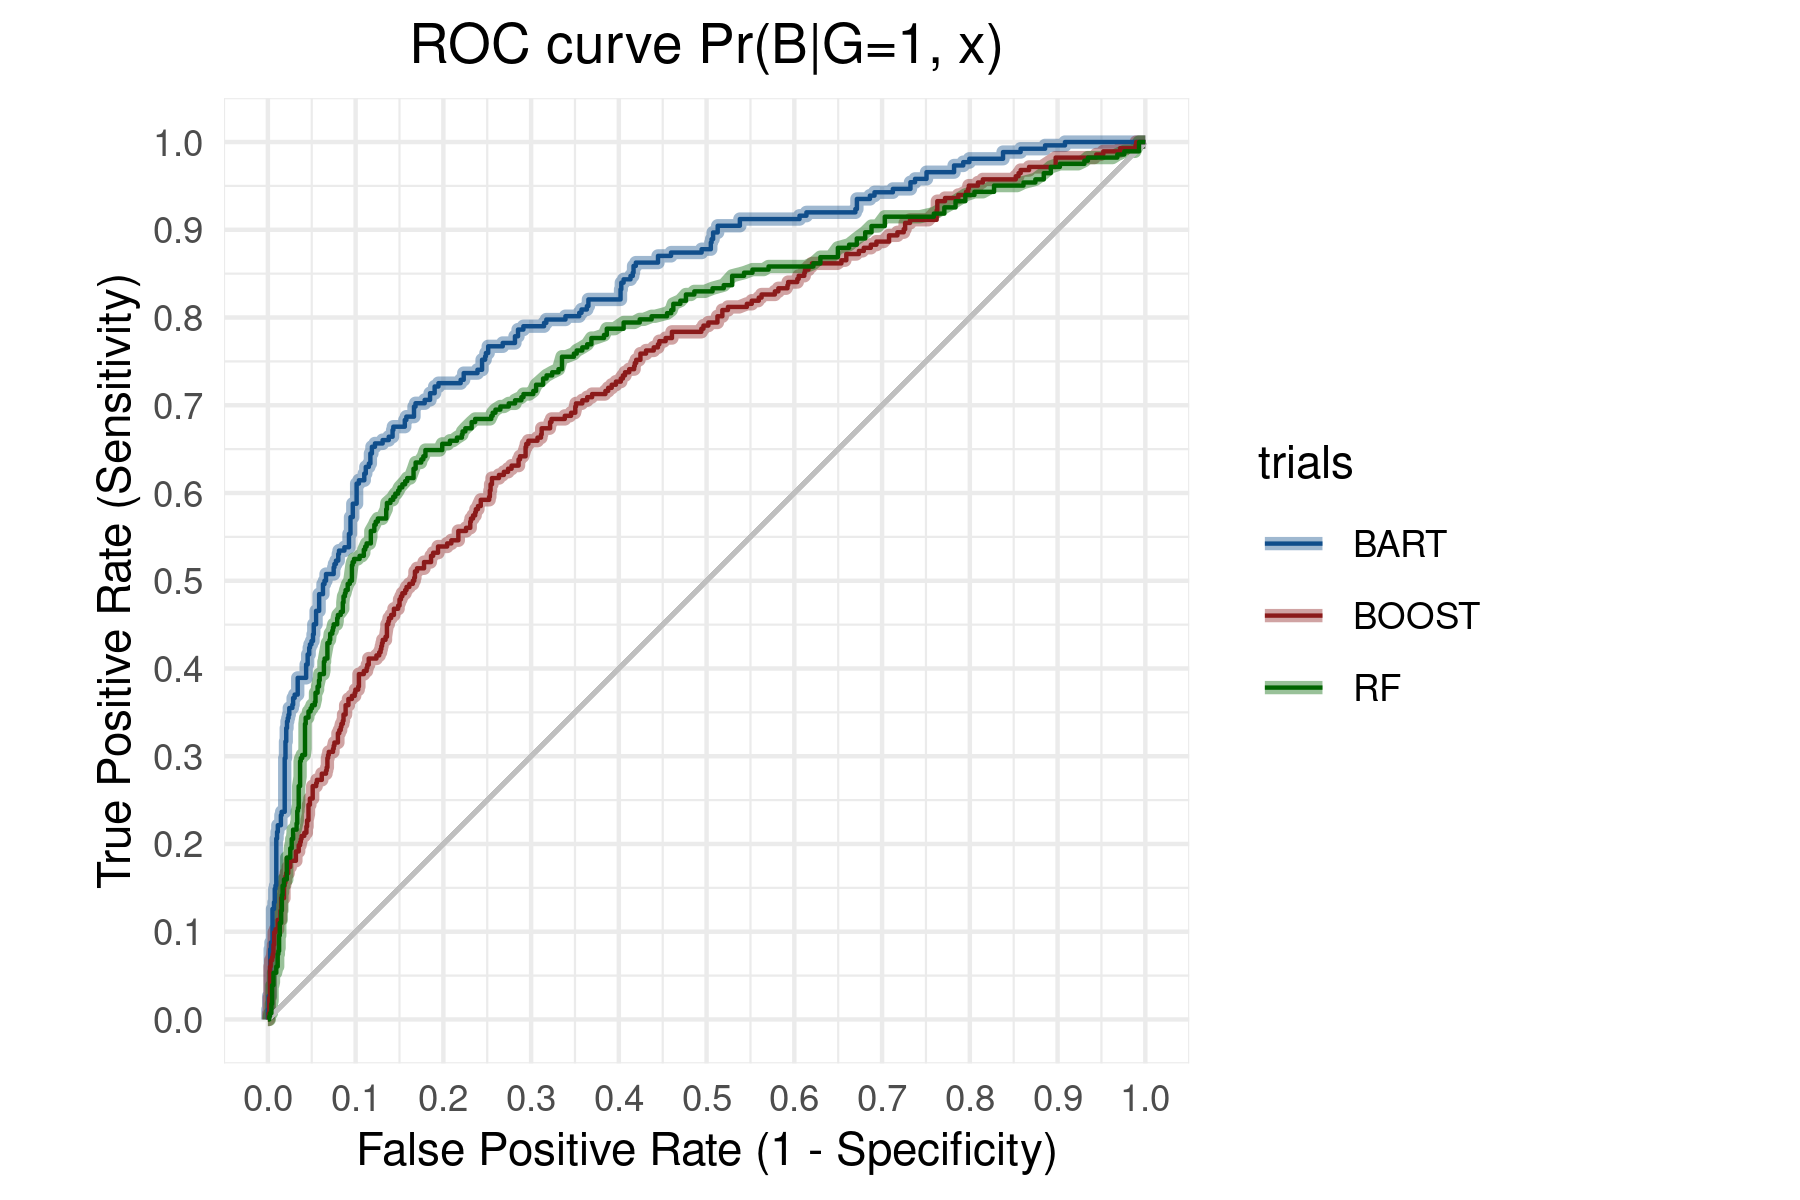
\includegraphics[width=8cm]{roc_pbg1_cv_png}
		
		
		
	\end{minipage}\hfill
	\begin{minipage}[t][-2.2cm][b]{.5\textwidth}	
		\centering
		%\begin{tabular}{lllll}%{P{1.6cm}P{1.5cm}P{1.5cm}P{1.5cm}P{1.5cm}P{2cm}}
		\begin{tabular}{P{1.1cm}P{1.2cm}P{1.25cm}P{1.25cm}}
			%	\toprule
			&\color{BrickRed}\textbf{XGBoost}&\color{darkgreen}\textbf{RanFor}&\color{navy}\textbf{BART}\\ \midrule
	
			
			Case   & AUC  & AUC & AUC  \\ \midrule
			$B_1, G_0$ &0.76&0.77&0.78\\ %\hline
			\rowcolor{navy!49!white}$B_1, G_1$ &0.79 &0.79&0.79 \\%\hline      
			$G_1$ &0.88&0.89&0.89 \\ \bottomrule%\\\midrule %\hline       
			%total&333&435&66&47&& \\ \bottomrule        
		\end{tabular}
		
		
	\end{minipage}
	\caption{Left: Area under curve of ROC plot, balanced 5-fold CV.  Plot of ROC performance for predicting $\Pr(B\mid G=1, \bm{x})$ .  Corresponds to shaded row in table on right.  Right:  case 1 is predicting bankruptcy when no going concern is issued, case 2 is when no concern issued, and case 3 predicts if concern is issued.  All the methods are \emph{similar}, with monotone BART seeming to be the top performer.}
	\label{roc_plot}
\end{figure}


	
	
	
	
\bibliography{sample}
	
	
	
	
	
\end{document}